
%-------------------------------------------------------------------------------
%-------------------------------------------------------------------------------
%-------------------------------------------------------------------------------
\chapter{DS2+ : X-ENS 2013}
%-------------------------------------------------------------------------------
%-------------------------------------------------------------------------------
%-------------------------------------------------------------------------------

On étudie dans ce problème un formalisme logique, la logique temporelle, permettant de définir des formules auxquelles
sont associés des langages de mots. Les mots décrivent l'évolution dans le temps d'un phénomène. Ainsi, pour toute formule $\varphi$ de la logique temporelle et pour tout mot $u$ on définira la
propriété que le mot $u$ satisfait la formule $\varphi$, et à toute formule $\varphi$ on associera l’ensemble $L_\varphi$ des mots qui satisfont $\varphi$.

L’objet principal de ce problème est de s’intéresser aux propriétés de ces langages $L_\varphi$.

La partie I introduit la logique temporelle et donne des exemples de formules. 

La partie II introduit une forme normale pour les formules. 

La partie III est consacrée à montrer que pour toute formule l’ensemble de mots associés est un langage
rationnel. 

Enfin, la partie IV étudie d’une part le problème de la satisfiabilité d’une formule (étant donnée une formule $\varphi$,
existe-t-il un mot satisfaisant $\varphi$ ?) et d’autre part l’expressivité des formules.


Les parties peuvent être traitées indépendamment. Néanmoins, chaque partie utilise des notations et des fonctions
introduites dans les parties précédentes.
%-------------------------------------------------------------------------------
%-------------------------------------------------------------------------------
%-------------------------------------------------------------------------------
\section{Préliminaires}
%-------------------------------------------------------------------------------
%-------------------------------------------------------------------------------
%-------------------------------------------------------------------------------
\begin{itemize}
\item Un {\bf alphabet} est un ensemble fini ${\cal A}$ dont les éléments sont appelés {\bf lettres}. 
\item Un {\bf } sur un alphabet ${\cal A}$ est une suite finie d’éléments de ${\cal A}$.
\item On notera $\varepsilon$ le mot vide (c’est-à-dire la suite vide).
\item On définira la longueur $|u|$ d’un mot non vide $u = a_0a_1\cdots a_{n-1}$ comme valant $n$. La longueur de $\varepsilon$ vaut 0.
\item Si ${\cal A}$ est un alphabet, on notera ${\cal A}^*$ l’ensemble des mots sur ${\cal A}$ et ${\cal A}^+={\cal A}^* \setminus \{\varepsilon\}$ l’ensemble des mots non vides sur ${\cal A}$.
\item Dans la suite, les lettres d’un mot de longueur $p$ sont indicées de 0 à $p-1$.
\item En OCaml, nous représenterons les mots à l’aide du type \type{string}. 
\item Si mot est de type \type{string} et $i$ est de type \type {int} alors \type{mot.[i]} est de type \type{char} et donne la lettre d’indice $i$ de mot . 

Par exemple \type{"bonjour".[3]} renvoie \type{'j'}.
\item La fonction \type{String.length} renvoie la longueur d’un mot.
\end{itemize}
%-------------------------------------------------------------------------------
Dans tout le problème on se fixe un alphabet fini ${\cal A}$ (on pourra imaginer qu’il s’agit des lettres minuscules de l’alphabet
usuel). 

On souhaite définir des ensembles de mots sur l’alphabet ${\cal A}$ à l’aide de formules logiques. Pour cela, on définit,
pour chaque lettre $a \in {\cal A}$, un prédicat $p_a$, qui permettra de tester si la lettre à une position qui sera donnée est un $a$. Pour construire des formules à partir de ces prédicats, on utilise les connecteurs booléens $\vee$ (ou), $\wedge$ (et) et $\neg$ (non) ainsi que les connecteurs temporels {\bf X} (juste après), {\bf G} (désormais), {\bf F} (un jour) et {\bf U} (jusqu’à).


Les formules de la logique temporelle sont alors construites par induction comme suit. Si $p_a$ est un prédicat, et si $\varphi$ et $\psi$ sont des formules de la logique temporelle, toutes les formules seront construites selon la syntaxe suivante :
%-------------------------------------------------------------------------------
\begin{enumerate}
    \item {\bf vrai}
    \item $p_a$
    \item $(\neg \varphi)$
    \item $(\varphi \vee \psi)$
    \item $(\varphi \wedge \psi)$
    \item $({\bf X} \varphi)$
    \item $({\bf G} \varphi)$
    \item $({\bf F} \varphi)$
    \item $(\varphi {\bf U} \psi)$
\end{enumerate}
%-------------------------------------------------------------------------------
Toutes les formules seront construites de la façon précédente, en omettant les parenthèses si celles-ci sont inutiles. Par
exemple, ${\bf X} p_b$, $p_a {\bf U} p_b$ et ${\bf F}({\bf G} p_a)$ sont des formules.

\medskip

Nous allons maintenant définir le sens (ou la sémantique) des formules.

Soit un mot $u$ et soit une formule de la logique temporelle $\varphi$. On définit, pour tout $i \ge 0$, la propriété "{\sf le mot $u$ satisfait la formule $\varphi$ à la position $i$}", ce qui sera noté $(u, i) \vDash \varphi$, comme suit. 

\begin{itemize}
\item Si $i \ge |u|$, on n’a pas $(u, i) \vDash \varphi$ : une formule ne peut être
vraie qu’à une position du mot ; en particulier le mot vide ne satisfait aucune formule (pas même la formule {\bf vrai}).
\item Si $i \le |u| - 1$, on note $u=a_0a_1\cdots a_{|u|-1}$ et on raisonne par induction sur la structure de $\varphi$.
\begin{enumerate}
    \item $(u, i) \vDash {\bf vrai}$.
    \item $(u, i) \vDash p_a$ si et seulement si $a_i=a$.
    \item $(u, i) \vDash (\neg \varphi)$ si et seulement si on n’a pas $(u, i) \vDash \varphi$.
    \item $(u, i) \vDash (\varphi \vee \psi)$ si et seulement si $(u, i) \vDash \varphi$ ou $(u, i) \vDash \psi$.
    \item $(u, i) \vDash (\varphi \wedge \psi)$ si et seulement si $(u, i) \vDash \varphi$ et $(u, i) \vDash \psi$.
    \item $(u, i) \vDash ({\bf X} \varphi)$ si et seulement si $(u, i+1) \vDash \varphi$. 
    
    Notez que si $i = |u| - 1$, alors on ne peut avoir $(u, i) \vDash ({\bf X} \varphi)$.
    \item $(u, i) \vDash ({\bf G} \varphi)$ si et seulement si $(u, j) \vDash \varphi$ pour tout $j$ tel que $i\le j < |u|$.
    \item $(u, i) \vDash ({\bf F} \varphi)$ si et seulement si il existe $j$ tel que $i\le j < |u|$ et $(u, j) \vDash \varphi$.
    \item $(u, i) \vDash (\varphi {\bf U} \psi)$ si et seulement si il existe $j$ tel que $i\le j < |u|$, $(u, j) \vDash \psi$ et $(u, k) \vDash \varphi$ pour tout $k\in\{i, i+1, \ldots, j-1\}$.
\end{enumerate}
\end{itemize}

On notera $(u, i) \vDash \varphi$ si et seulement si l’on n’a pas $(u, i) \vDash \varphi$. 

On notera $u \vDash \varphi$  (et on dira alors que $\varphi$ est vraie pour $u$) le fait que $(u, 0) \vDash \varphi$ .
On notera $u \nvDash \varphi$  le fait que $(u, 0) \nvDash \varphi$ .

{\bf Exemples}
\begin{itemize}
    \item $(aaabcbab, 2) \vDash ({\bf X} p_b)$ car la lettre d’indice 3 de $aaabcbab$ est un $b$.
    \item $aaabcbab \vDash (p_a{\bf U} p_b)$ car la lettre d’indice 3 est un $b$ et n'est précédée que de $a$.
    \item $aaabcbab \vDash {\bf F}({\bf G} p_a)$ car il n’existe pas d’indice à partir duquel il n’y ait plus que des $a$ (en effet, la dernière lettre est un $b$).
\end{itemize}

%-------------------------------------------------------------------------------
%-------------------------------------------------------------------------------
\begin{Exercise}\it
On pose $u=bbbcbbaa$. 
Pour chacun des énoncés ci-dessous dire s'il est vrai en justifiant brièvement votre réponse.
\begin{enumerate}
  \item $(u,4)\vDash{\bf G}(p_a\vee p_b)$
  \item $(u,2)\vDash{\bf X}({\bf G}(p_a\vee p_c))$
  \item $(u,1)\vDash{\bf F}({\bf G}(p_a\vee p_b))$
  \item $u\vDash(p_a\vee p_b){\bf U}(p_a\vee p_c)$
\end{enumerate}
\end{Exercise}
%-------------------------------------------------------------------------------
\begin{Answer}
\begin{enumerate}
\item $(u, 4) \vDash  {\bf G}(p_a \vee p_b )$  est vrai car les lettres sont $a$ ou $b$ à partir du rang 4.
\item $(u, 2) \vDash {\bf X}\bigl({\bf G}(p_a \vee p_c )\bigr)$ signifie $(u, 3) \vDash  {\bf G}(p_a \vee p_c)$ qui est faux car $u_4$ est $b$.
\item Comme $(u, 4) \vDash  {\bf G}(p_a \vee p_b )$  est vrai alors $(u, 2) \models  {\bf F}\bigl({\bf G}(p_a \vee p_b )\bigr)$  est vrai.
\item $u \vDash (p_a \vee p_b ){\bf U}(p_a \vee p_c )$ est vrai car $(u, j) \vDash p_b$ pour $j  \le  2$ et $(u, 3) \models p_c$.
\end{enumerate}
\end{Answer}
%-------------------------------------------------------------------------------
\newpage
%-------------------------------------------------------------------------------
\begin{Exercise}\it
Écrire une formule $\varphi$ telle que $u\vDash \varphi$ si et seulement si $u$ contient un $a$ suivi plus tard d'un $b$. Par exemple on aura $ccacccba\vDash \varphi$ tandis que $ccacccaa\nvDash \varphi$.
\end{Exercise}
%-------------------------------------------------------------------------------
\begin{Answer}
La formule ${\bf F}\bigl(p_a \wedge {\bf F}(p_b)\bigr)$ convient.
\end{Answer}
%-------------------------------------------------------------------------------
\medskip
%-------------------------------------------------------------------------------
\begin{Exercise}\it
Écrire une formule ${\bf fin}$ telle que $(u,i)\vDash {\bf fin}$ si et seulement si $i=|u|-1$ (c'est-à-dire si et seulement si $i$ est l'indice de la dernière lettre de $u$).
\end{Exercise}
%-------------------------------------------------------------------------------
\begin{Answer}
Un indice $i$ est valide pour un mot $u$ si et seulement si $(u,i) \vDash {\bf vrai}$.

Le dernier indice valide d'un mot $u$ est l'indice valide tel que son successeur ne l'est pas, il est donc caractérisé par 
${\bf fin} = {\bf vrai} \wedge \neg {\bf X}({\bf vrai})$
\end{Answer}
%-------------------------------------------------------------------------------
%-------------------------------------------------------------------------------
Dans la suite, on pourra utiliser ${\bf fin}$ comme une boîte noire.

%-------------------------------------------------------------------------------
%-------------------------------------------------------------------------------
\begin{Exercise}\it
Écrire une formule $\varphi$ telle que $u\vDash \varphi$ si et seulement si $u$ se termine par un $a$.
\end{Exercise}
%-------------------------------------------------------------------------------
\begin{Answer}
$u$ se termine par $a$ si et seulement si la dernière lettre est $a$. Il doit donc exister une lettre qui est finale et qui vaut $a$ : ${\bf F}(\text{Fin} \wedge p_a)$.

On peut aussi exprimer qu'il y un $a$ qui suit chaque position, en particulier la dernière. 

On aboutit à la formule ${\bf G}\bigl({\bf F}(p_a)\bigr)$.
\end{Answer}
%-------------------------------------------------------------------------------
%-------------------------------------------------------------------------------
\begin{Exercise}\it
Écrire une formule $\varphi$ telle que $u\vDash\varphi$ si et seulement si $u=ababab\cdots ab$, c'est-à-dire si et seulement s'il existe $k \ge 1$ tel que $u=u_0u_1\cdots u_{2k-1}$ et, pour tout $i$ tel que $0\le i < 2k$ on a $u_i =a$ si $i$ est pair et $u_i =b$ si $i$ est impair.
\end{Exercise}
%-------------------------------------------------------------------------------
\begin{Answer}
La périodicité s'exprime par le fait que, pour toute lettre, selon qu'elle vaille $a$ ou $b$ la suivante vaut $b$ ou $a$ ; chaque lettre vérifie $(p_a \wedge {\bf X}(p_b))$ ou $(p_b \wedge {\bf X}(p_a))$. La dernière lettre, qui est un $b$ ne vérifie pas $(p_b \wedge {\bf X}(p_a))$, il faut ajouter la condition $p_b \wedge \text{Fin}$.

De plus, la première lettre doit être un $a$. 

Le mot doit donc vérifier $p_a\wedge {\bf G}\bigl((p_a \wedge {\bf X}(p_b)) \vee (p_b \wedge {\bf X}(p_a)) \vee (p_b \wedge \text{Fin})\bigr)$.

\end{Answer}
%-------------------------------------------------------------------------------
%-------------------------------------------------------------------------------
\begin{Exercise}[title = {Pour les cubes seulement}]\it
Pour cette question, on pose ${\cal A}=\{a, b, c\}$. Soit $\varphi={\bf F}\bigl(p_a \wedge {\bf X}\bigl({\bf G}(\neg p_a)\bigr)\wedge {\bf F}(p_b \wedge {\bf X} p_c)\bigr)$. Décrire un automate fini (pouvant être non-déterministe) reconnaissant le langage $L_\varphi=\bigl\{u\in {\cal A}^+\bigm|u\vDash \varphi\bigr\}$.
\end{Exercise}
%-------------------------------------------------------------------------------
\begin{Answer}
On veut les mots qui contiennent un $a$ suivi uniquement de $b$ et $c$, avec dans cette suite l'apparition d'un $bc$.

Une expression régulière associée est $(a+b+c)^*.a.b^*.b.c.(b+c)^*$.

Un automate qui reconnaît le langage peut être

\begin{center}
\begin{tikzpicture}[node distance=18mm,
                    >=latex,
                    accepting=accepting by gdouble,
                    initial text =
                    ] 
 \node[state,initial] (s0) {};
 \node[state] (s1) [right=of s0] {};
 \node[state] (s2) [right=of s1] {};
 \node[state,accepting] (s3) [right=of s2] {};
 \path[->] (s0) edge node[above] {$a$} (s1)
                edge[loop above] node [above] {$a,b,c$}()
           (s1) edge node[above] {$b$} (s2)
                edge [loop above] node[above] {$b$} ()
                edge [loop below] node[below] {$c$} ()
           (s2) edge node[above] {$c$} (s3)
           (s3) edge [loop above] node [above] {$b$}()
                edge [loop below] node [below] {$c$}();
\end{tikzpicture}
\end{center}
\end{Answer}
%-------------------------------------------------------------------------------
%-------------------------------------------------------------------------------

\medskip

Deux formules $\varphi$ et $\psi$ sont {\bf équivalentes}, ce que l'on note $\varphi \equiv \psi$, si pour tout mot $u$, on a 

$u\vDash \varphi$ si et seulement si $u\vDash \psi$. Autrement dit, les formules $\varphi$ et $\psi$ sont vraies pour les mêmes mots.
%-------------------------------------------------------------------------------
%-------------------------------------------------------------------------------
\begin{Exercise}\it
Soient $\varphi$ et $\psi$ deux formules quelconques. Montrer que l'on a $\varphi {\bf U} \psi \equiv \psi \vee  \bigl(\varphi \wedge  \bigl({\bf X}(\varphi {\bf U} \psi)\bigr)\bigr)$.
\end{Exercise}
%-------------------------------------------------------------------------------
\begin{Answer}
On définit les nouveaux connecteurs $U_j$ par la sémantique $(u,i) \vDash \varphi {\bf U_j} \psi$ si et seulement si $(u,j) \vDash \psi$ et $(u,k) \vDash \varphi$ pour $i\le k< j$.

On remarque que $(u,i) \vDash \varphi {\bf U_i} \psi$ se traduit par $(u,i) \vDash \psi$ et, pour $i <j$,

$(u,i) \vDash \varphi {\bf U_j} \psi$ se traduit par $(u,i) \vDash \varphi$ et $(u,i+1) \vDash \varphi {\bf U_j} \psi$, c'est-à-dire, $(u,i) \vDash {\bf X}(\varphi {\bf U_j} \psi)$.

\medskip

Comme la définition de $(u,i) \vDash \varphi U \psi$ peut se lire sous la forme

$(u,i) \vDash \varphi U_i \psi$ ou il existe $j$ tel que $i+1 \le j < |u|$ et $(u,i) \vDash \varphi U_j \psi$ on obtient

\[\varphi U \psi \equiv \psi \vee \bigl(\varphi \wedge {\bf X}(\varphi U \psi)\bigr)\]
\newpage
\end{Answer}
%-------------------------------------------------------------------------------
%-------------------------------------------------------------------------------
%-------------------------------------------------------------------------------
\section{Normalisation de formules}
%-------------------------------------------------------------------------------
%-------------------------------------------------------------------------------
%-------------------------------------------------------------------------------
Afin de manipuler des formules de la logique temporelle, on va représenter ces dernières par des arbres. Outre les prédicats $(p_a)_{a\in A}$ et la formule ${\bf vrai}$ nous avons des connecteurs unaires $(\neg, {\bf X}, {\bf G} \text{ et }{\bf F})$ et des connecteurs binaires $(\vee, \wedge \text{ et }{\bf U})$. À la manière des expressions arithmétiques, on représente une formule de la logique temporelle par un arbre dont les feuilles sont étiquetées soit par un prédicat $p_a$ soit par ${\bf vrai}$, et dont les nœuds internes sont étiquetés par un connecteur unaire (un tel nœud aura alors un seul fils) ou par un connecteur binaire (un tel nœud aura alors deux fils). Dans la suite, on confondra fréquemment une formule avec sa représentation par un arbre.

Par exemple, la formule $\bigl({\bf F}({\bf G}(p_a\vee p_b))\bigr) \wedge p_b$ sera représentée par l'arbre ci-dessous :
%-------------------------------------------------------------------------------
\begin{center}
\begin{tikzpicture}[level distance=9mm, sibling distance=15mm]
\node{$\wedge$}
  child {node {${\bf F}$}
    child{node {${\bf G}$}
      child {node {$\vee$}
        child {node {$p_a$}}
        child {node {$p_b$}}}}}
  child {node {$p_b$}} ;
\end{tikzpicture}
\end{center}
%-------------------------------------------------------------------------------

\newpage

On définit le type suivant pour les formules
%-------------------------------------------------------------------------------
\begin{lstlisting}
type formule =  VRAI
               |Predicat of char
               |NON of formule
               |ET of formule * formule
               |OU of formule * formule
               |X of formule
               |G of formule
               |F of formule
               |U of formule * formule ;;
\end{lstlisting}
%-------------------------------------------------------------------------------

On définit la taille d'une formule par le nombre de nœuds (y compris les feuilles) de l'arbre qui la représente.

En particulier, la formule ${\bf vrai}$ et les formules réduites à un prédicat $p_a$ sont de taille 1.

%-------------------------------------------------------------------------------
%-------------------------------------------------------------------------------
\begin{Exercise}\it
Écrire une fonction \type{taille} qui prend en argument une formule et renvoie sa taille. 
\begin{lstlisting}
taille: formule -> int
\end{lstlisting}
\end{Exercise}
%-------------------------------------------------------------------------------
\begin{Answer}
On doit séparer selon les motifs :
\begin{lstlisting}
let rec taille form = 
   match form with 
   |VRAI -> 1
   |Predicat(_) -> 1
   |NON f -> 1 + taille f
   |ET (fg, fd) -> 1 + taille fg + taille fd
   |OU (fg, fd) -> 1 + taille fg + taille fd
   |X f -> 1 + taille f
   |G f -> 1 + taille f 
   |F f -> 1 + taille f
   |U (fg, fd) -> 1 + taille fg + taille fd;;
\end{lstlisting} 
Dans la suite on notera $|\varphi|$ la taille d'une formule $\varphi$.
\end{Answer}
%-------------------------------------------------------------------------------
%-------------------------------------------------------------------------------
\begin{Exercise}\it
Donner, pour toute formule $\varphi$ n'utilisant pas le connecteur ${\bf F}$, une formule équivalente à $({\bf F}\varphi)$ qui n'utilise pas le connecteur temporel ${\bf F}$. 

En déduire une fonction \type{normaliseF} qui prend en entrée une formule quelconque et renvoie une formule équivalente qui n'utilise pas le connecteur ${\bf F}$. 

Quelle est la complexité de votre algorithme ?
\begin{lstlisting}
normaliseF: formule -> formule
\end{lstlisting}
\end{Exercise}
%-------------------------------------------------------------------------------
\begin{Answer}
$(u,i) \vDash {\bf F}(\varphi)$ signifie qu'il existe un entier $j\ge i$, valide pour $u$, tel que $(u,j) \vDash \varphi$.
Pour $i\le k < j$ on a $(u,i) \vDash{\bf vrai}$ donc ${\bf F}(\varphi) \equiv {\bf vrai}\,{\bf U}\varphi$.

\begin{lstlisting}
let rec normaliseF form = 
   match form with 
   |VRAI -> VRAI
   |Predicat k -> Predicat k
   |NON f -> NON(normaliseF f)
   |ET (fg,fd) -> ET(normaliseF fg, normaliseF fd)
   |OU (fg,fd) -> OU(normaliseF fg, normaliseF fd)
   |X f -> X (normaliseF f)
   |G f -> G (normaliseF f)
   |F f -> U (VRAI, normaliseF f)
   |U (fg,fd) -> U (normaliseF fg, normaliseF fd);;
\end{lstlisting} 

L'algorithme termine car chaque appel récursif est fait sur une formule de taille strictement inférieure : on doit aboutir aux cas élémentaires.

La complexité est linéaire car les formules ci-dessus permettent de majorer la complexité par la taille ; elle est un ${\cal O}\bigl(|\varphi|\bigr)$.
\end{Answer}
%-------------------------------------------------------------------------------
%-------------------------------------------------------------------------------

\medskip

Une formule qui utilise comme seuls connecteurs temporels le ${\bf X}$ et le ${\bf U}$ sera qualifiée de {\bf normalisée}.

%-------------------------------------------------------------------------------
%-------------------------------------------------------------------------------
\begin{Exercise}\it
Montrer que toute formule est équivalente à une formule normalisée. Donner une fonction \type{normalise} de complexité linéaire qui prend en entrée une formule quelconque et renvoie une formule équivalente normalisée.
\begin{lstlisting}
normalise: formule -> formule
\end{lstlisting}
\end{Exercise}
%-------------------------------------------------------------------------------
\begin{Answer}

On peut remarquer qu'on a ${\bf G}(\varphi) \equiv \varphi\, {\bf U} (\varphi \wedge \text{Fin}) \equiv  
\varphi\, {\bf U} (\varphi \wedge {\bf vrai} \wedge {\bf X}(\neg {\bf vrai}))$.

On peut trouver plus simple en remarquant que {\bf G} est une double négation de {\bf F} :
${\bf G}(\varphi) \equiv \neg\bigl(F(\neg \varphi)\bigr)$, avec la formule ci-dessus on obtient

\[{\bf G}(\varphi) \equiv \neg\bigl( {\bf vrai} {\bf U}(\neg \varphi)\bigr)\]

On peut utiliser ces formules pour éliminer les {\bf G} puis éliminer les {\bf F} en même temps.

\begin{lstlisting}
let rec normalise form = 
   match form with 
   |VRAI -> VRAI
   |Predicat k-> Predicat k
   |NON f -> NON (normalise f)
   |ET (fg, fd) -> ET (normalise fg, normalise fd)
   |OU (fg, fd) -> OU(normalise fg, normalise fd)
   |X f -> X (normalise f)
   |G f -> NON(U (VRAI, NON (normalise f)))
   |F f -> U (VRAI, normaliseF f)
   |U (fg, fd) -> U (normalise fg, normalise fd);;
\end{lstlisting} 

Comme ci-dessus la terminaison et la complexité linéaire proviennent de la majoration du nombre d'instruction par la taille de l'arbre.
\end{Answer}
%-------------------------------------------------------------------------------
%-------------------------------------------------------------------------------
Dans toute la suite du problème, on supposera que l'on travaille avec des {\bf formules normalisées}.

%-------------------------------------------------------------------------------
%-------------------------------------------------------------------------------
\begin{Exercise}\it
Écrire une fonction récursive \type{veriteN} qui prend en argument un mot $u$, un indice $i$ et une formule (normalisée) $\varphi$ et détermine si $(u, i)\vDash \varphi$. Justifier que votre fonction termine et indiquer si elle est exponentielle ou polynomiale en la taille de ses arguments.
\begin{lstlisting}
veriteN: string -> int -> formule -> bool
\end{lstlisting}
\end{Exercise}
%-------------------------------------------------------------------------------
\begin{Answer} On utilise la question {\bf 7}.
\begin{lstlisting}
let rec veriteN u i form = 
   let n = String.length u in
   if i >= n || i < 0
   then false
   else match form with 
      |VRAI -> true
      |Predicat k -> u.[i] = k
      |NON f -> not (veriteN u i f)
      |ET (fg, fd) -> (veriteN u i fg) && (veriteN u i fd)
      |OU (fg, fd) -> (veriteN u i fg) || (veriteN u i fd)
      |X f -> veriteN u (i+1) f
      |U (fg, fd) ->   (veriteN u i fd) 
                    || (veriteN u i fg) && (veriteN u (i+1) form)
      |_ -> failwith "Formule non normalisée";;
\end{lstlisting} 



Dans chaque cas on appelle récursivement {\tt veriteN} à une ou plusieurs formules qui sont soit de taille strictement inférieure, soit  avec un mot de longueur strictement inférieure en considérant que {\tt (u,i)} représente en fait le suffixe de $u$ obtenu en lui enlevant $i$ lettres. Ainsi la somme $|u|+|\varphi|$ est strictement décroissante donc on aboutit donc à une formule atomique ou à un mot vide et, dans ces deux cas, la récursivité s'arrête. L'algorithme termine.

On note $C(p,\varphi)$ la complexité du calcul de {\tt veriteN u i phi} avec $|u| = p + i$.

Si $\varphi = \varphi_1\, {\bf U}\, \varphi_2$ on a $C(p,\varphi)= C(p,\varphi_1)+C(p,\varphi_2)+C(p-1,\varphi)+2$.

Comme $C(0,\varphi)=0$ on en déduit que $\displaystyle C(p,\varphi)=\sum_{k=1}^{p} \bigl(C(k,\varphi_1)+C(k,\varphi_2)+2\bigr)$.

On définit $\psi_r$ par $\psi_1=p_a$ et $\psi_r=p_a\,{\bf U}\, \psi_{r-1}$ et $\gamma(p,r) = C(p,\psi_r)$.

La formule ci-dessus donne $\displaystyle \gamma(p,r) = \sum_{k=1}^{p} \bigl(\gamma(k,r-1)+3\bigr)$ avec $\gamma(p,1)=1$.

On a donc $\gamma(p,2)=4p$, $\gamma(p,3)=2p^2+5p$ et on montre par récurrence que $\gamma(p,r)$ est un polynôme de de degré $r-1$ en $p$.
Comme la taille de $\psi_r$ est $2r-1$ on a une complexité équivalente à $Kp^{(|\psi_r|-1)/2}$ exponentielle en la taille.

Dans le cas général la complexité est donc au moins exponentielle en la taille.
\end{Answer}
%-------------------------------------------------------------------------------
\newpage
%-------------------------------------------------------------------------------
%-------------------------------------------------------------------------------
\section{Rationalité des langages décrits par des formules}
%-------------------------------------------------------------------------------
%-------------------------------------------------------------------------------
%-------------------------------------------------------------------------------
Le but de cette partie est de montrer qu'étant donnée une formule $\varphi$, l'ensemble des mots pour lesquels $\varphi$ est vraie est un langage rationnel.

\smallbreak

Soit $\varphi$ une formule représentée par un arbre $t_\varphi$. Une {\bf sous-formule} de $\varphi$ est une formule représentée par un sous-arbre de $t_\varphi$. Par exemple si l'on considère la formule $\varphi=({\bf X}({\bf X}(p_a {\bf U} p_b)))\wedge p_b$, représentée par l'arbre ci-dessous,
%-------------------------------------------------------------------------------
\begin{center}
\begin{tikzpicture}[level distance=9mm, sibling distance=15mm]
\node{$\wedge$}
  child {node {${\bf X}$}
    child{node {${\bf X}$}
      child {node {${\bf U}$}
        child {node {$p_a$}}
        child {node {$p_b$}}}}}
  child {node {$p_b$}} ;
\end{tikzpicture}
\end{center}
%-------------------------------------------------------------------------------
l'ensemble de ses sous-formules est :
\[\bigl\{({\bf X}({\bf X}(p_a{\bf U} p_b)))\wedge p_b,\ {\bf X}({\bf X}(p_a{\bf U} p_b)),\ {\bf X}(p_a{\bf U} p_b),\ p_a{\bf U} p_b,\ p_b,\ p_a \bigr\}\]

On souhaite représenter des ensembles de sous-formules d'une formule donnée. Pour cela, on va utiliser des arbres dont les nœuds sont étiquetés (en plus des symboles de la logique) par des booléens. Par exemple pour la formule $({\bf X}({\bf X}(p_a {\bf U} p_b))) \wedge p_b$ représentée ci-dessus, l'ensemble de sous-formules $\{p_a,\ {\bf X}(p_a {\bf U} p_b)\}$ sera représenté par l'arbre ci-dessous.
%-------------------------------------------------------------------------------
\begin{center}
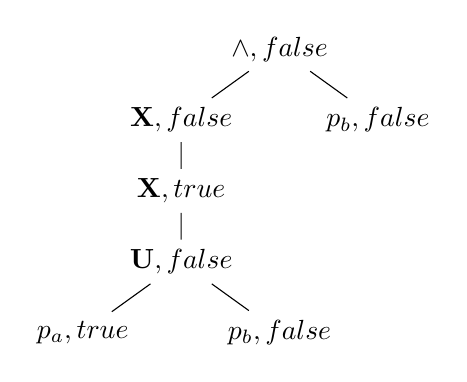
\begin{tikzpicture}[level distance=9mm, sibling distance=25mm]
\node{$\wedge, \type{false}$}
  child {node {${\bf X}, \type{false}$}
    child{node {${\bf X}, \type{true}$}
      child {node {${\bf U}, \type{false}$}
        child {node {$p_a, \type{true}$}}
        child {node {$p_b, \type{false}$}}}}}
  child {node {$p_b, \type{false}$}} ;
\end{tikzpicture}
\end{center}
%-------------------------------------------------------------------------------

Une sous-formule $\psi$ appartient à l'ensemble représenté par un arbre de type \type{ensemble} s'il existe un nœud de l'arbre étiqueté par \type{true} et dont le sous-arbre «correspond» à la formule $\psi$ (c'est-à-dire qu'après suppression des booléens, le sous-arbre est égal à l'arbre codant $\psi$). Le type \type{ensemble} est défini comme suit.
%-------------------------------------------------------------------------------
\begin{lstlisting}
type ensemble = eformule * bool
 and eformule =  AVRAI
                |APredicat of char
                |ANON of ensemble
                |AET of ensemble * ensemble
                |AOU of ensemble * ensemble
                |AX of ensemble 
                |AU of ensemble * ensemble ;;
\end{lstlisting}
%-------------------------------------------------------------------------------

On rappelle que l'on ne travaille plus qu'avec des formules normalisées.

Si $a$ est une lettre et si $u$ est un mot, on note $a\cdot u$ le mot obtenu en ajoutant $a$ en tête de $u$. Si $u = a_0a_1\cdots a_{p-1}$, alors $v =aa_0a_1\cdots a_{p-1}$.

\newpage
%-------------------------------------------------------------------------------
%-------------------------------------------------------------------------------
\begin{Exercise}\it
Écrire une fonction \type{initialise} qui prend en argument une formule $\varphi$ et renvoie un ensemble représentant l'ensemble vide de sous-formules de $\varphi$. 
\begin{lstlisting}
initialise: formule -> ensemble
\end{lstlisting}
\end{Exercise}
%-------------------------------------------------------------------------------
\begin{Answer}
Il suffit de convertir l’arbre de la formule en arbre-ensemble en marquant par faux chaque nœud.
\begin{lstlisting}
let rec initialise form = 
   match form with 
   |VRAI -> AVRAI, false
   |Predicat k -> APredicat k, false
   |NON f -> ANON(initialise f), false
   |ET (fg, fd) -> AET (initialise fg, initialise fd), false
   |OU (fg, fd) -> AOU (initialise fg, initialise fd), false
   |X f -> AX (initialise f), false
   |U (fg, fd) -> AU (initialise fg, initialise fd), false
   |_ -> failwith "Formule non normalisée";;
\end{lstlisting} 
\end{Answer}
%-------------------------------------------------------------------------------
%-------------------------------------------------------------------------------
\begin{Exercise}\it
Soient $u$ un mot, $\varphi$ une formule et $\cal S$ l'ensemble des sous-formules de $\varphi$ vraies pour $u$. Soit $a$ une lettre. Montrer que l'ensemble $\cal S'$ des sous-formules de $\varphi$ vraies pour $a\cdot u$ peut être déterminé uniquement en fonction de $a$ et de $\cal S$ (en particulier indépendamment de $u$).
\end{Exercise}
%-------------------------------------------------------------------------------
\begin{Answer}
Soit  une formule normalisée $\varphi$ ; on montre par induction structurelle que l'appartenance de $\varphi$ à $\cal S'$ dépend uniquement de $a$ et de $\cal S$.

C'est vrai pour les formules "terminales" :

\begin{itemize}[itemindent=*, leftmargin=0pt]
  \item Si $\varphi={\bf vrai}$, alors $\varphi$ appartient toujours à $\cal S'$ car $a\cdot u$ n'est pas vide.
  \item Si $\varphi=p_x$ alors $\varphi$ appartient à $\cal S'$ si et seulement si $a = x$.
\end{itemize}

On suppose que l'appartenance de $\varphi_1$, $\varphi_2$ et $\psi$ à ${\cal S}'$ ne dépend que $a$ et de ${\cal S}$.

\begin{itemize}[itemindent=*, leftmargin=0pt]
  \item Si $\varphi=\neg\psi$ alors $\varphi$ appartient à $\cal S'$ si et seulement si $\psi$ n'appartient pas à $\cal S'$.
  \item Si $\varphi=\psi_1\wedge\psi_2$, alors $\varphi$ appartient à $\cal S'$ si et seulement si $\psi_1$ et $\psi_2$ appartiennent à $\cal S'$.
  \item Si $\varphi=\psi_1\vee\psi_2$, alors $\varphi$ appartient à $\cal S'$ si et seulement si $\psi_1$ ou $\psi_2$ appartient à $\cal S'$.
  \item Si $\varphi={\bf X}\psi$, alors $\varphi$ appartient à $\cal S'$ si et seulement si $\psi$ appartient à $\cal S$.
  \item si $\varphi=\psi_1{\bf U}\psi_2$, alors $\varphi$ appartient à $\cal S'$ si et seulement $\psi_2$ appartient à $\cal S'$ ou $\psi_1$ appartient à $\cal S'$ et $\varphi$ appartient à $\cal S$.
\end{itemize}

Dans tous les cas on voit que l'appartenance de $\varphi$ à ${\cal S}'$ ne dépend que de $a$ et de $\cal S$.
\end{Answer}
%-------------------------------------------------------------------------------
%-------------------------------------------------------------------------------
\begin{Exercise}\it
En vous basant sur la question 13, écrire une fonction \type{maj} qui prend en argument un \type{ensemble} $\cal S$ (représentant un ensemble de sous-formules d'une formule $\varphi$) et une lettre $a$ et renvoie un \type{ensemble} $\cal S'$ tel que : pour tout mot $u$ si $\cal S$ représente l'ensemble $\bigl\{\psi\bigm|u\vDash \psi\text{ et }\psi \text{ sous-formule de $\varphi$}\bigr\}$ des sous-formules de $\varphi$ vraies pour $u$ alors $\cal S'$ représente l'ensemble $\bigl\{\psi\bigm|a\cdot u\vDash \psi\text{ et }\psi \text{ sous-formule de $\varphi$}\bigr\}$ des sous-formules de $\varphi$ vraies pour $a\cdot u$.
Justifier la terminaison et préciser la complexité (dans la taille de la formule) de votre fonction.
\end{Exercise}
%-------------------------------------------------------------------------------
\begin{Answer}
On agit selon la première composante du couple
\begin{lstlisting}
let rec maj ens a = 
   match (fst ens) with
   |AVRAI -> AVRAI, true
   |APredicat k -> APredicat k, a = k
   |ANON f -> let s, b = maj f a in ANON (s, b), not b
   |AET (fg, fd) -> let sg,bg = maj fg a and sd,bd = maj fd a
                    in AET ((sg, bg), (sd, bd)), bg && bd
   |AOU (fg, fd) -> let sg,bg = maj fg a and sd,bd = maj fd a
                    in AET ((sg, bg), (sd, bd)), bg || bd
   |AX f -> let s = maj f a in AX s, (snd ens)
   |AU (fg, fd) -> let sg,bg = maj fg a and sd,bd = maj fd a
                   in AU ((sg, bg), (sd, bd)),
                          (bd || bg && (snd ens)) ;;
\end{lstlisting}
\end{Answer}
%-------------------------------------------------------------------------------
%-------------------------------------------------------------------------------

Par exemple si l'on reprend l'exemple de la formule $\varphi=({\bf X}({\bf X}(p_a {\bf U} p_b))) \wedge p_b$ (arbre à gauche ci-dessous) et de l'\type{ensemble} $\cal S$ (au centre ci-dessous), alors \type{maj S `b`} devra renvoyer l'ensemble $\cal S'$ (à droite ci-dessous).
%-------------------------------------------------------------------------------
\medskip

\begin{center}
\begin{tikzpicture}[level distance=9mm, sibling distance=15mm]
\node{$\wedge$}
  child {node {${\bf X}$}
    child{node {${\bf X}$}
      child {node {${\bf U}$}
        child {node {$p_a$}}
        child {node {$p_b$}}}}}
  child {node {$p_b$}} ;
\end{tikzpicture}
\ 
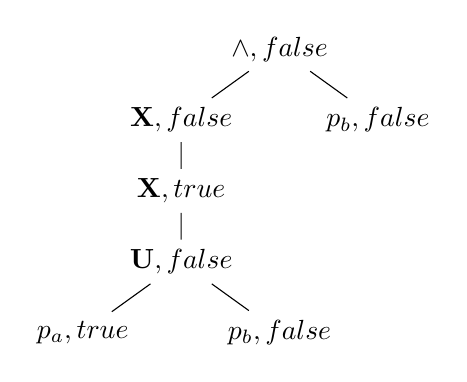
\begin{tikzpicture}[level distance=9mm, sibling distance=25mm]
\node{$\wedge, \type{false}$}
  child {node {${\bf X}, \type{false}$}
    child{node {${\bf X}, \type{true}$}
      child {node {${\bf U}, \type{false}$}
        child {node {$p_a, \type{true}$}}
        child {node {$p_b, \type{false}$}}}}}
  child {node {$p_b, \type{false}$}} ;
\end{tikzpicture}
\qquad
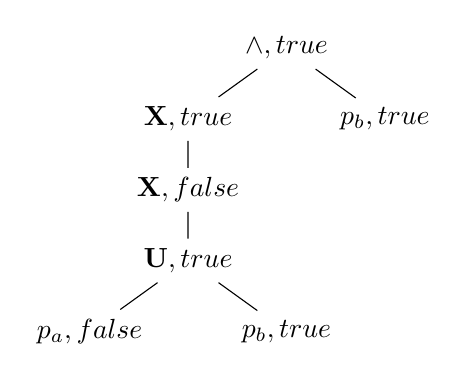
\begin{tikzpicture}[level distance=9mm, sibling distance=25mm]
\node{$\wedge, \type{true}$}
  child {node {${\bf X}, \type{true}$}
    child{node {${\bf X}, \type{false}$}
      child {node {${\bf U}, \type{true}$}
        child {node {$p_a, \type{false}$}}
        child {node {$p_b, \type{true}$}}}}}
  child {node {$p_b, \type{true}$}} ;
\end{tikzpicture}
\end{center}
%-------------------------------------------------------------------------------
\begin{lstlisting}
maj: ensemble -> char -> ensemble
\end{lstlisting}
%-------------------------------------------------------------------------------
%-------------------------------------------------------------------------------
\begin{Exercise}\it
Écrire une fonction \type{sousFormulesVraies} qui prend en argument une formule $\varphi$ et un mot et renvoie un \type{ensemble} décrivant les sous-formules $\psi$ de $\varphi$ telles que $u\vDash \psi$. Votre fonction devra avoir une complexité polynomiale dans la taille de la formule et dans la taille du mot. Justifier la terminaison et préciser la complexité (dans la taille de la formule et la taille du mot).
\begin{lstlisting}
sousFormulesVraies: formule -> string -> ensemble
\end{lstlisting}
\end{Exercise}
%-------------------------------------------------------------------------------
\begin{Answer}
On construit l'ensemble à partir de l'ensemble associé au mot vide, celui construit à la question 12, puis en ajoutant les lettres une-par-une depuis la dernière. On doit donc lire le mot de droite à gauche.

\begin{lstlisting}
let sousFormulesVraies form u = 
  let ens = ref (initialise form) in 
  let n = String.length u in
  for i = (n-1) downto 0 do 
    ens := maj !ens (u.[i]) done;
  !ens;;
\end{lstlisting}

La fonction {\tt maj} termine et a une complexité en ${\cal O}\bigl(|\varphi|\bigr)$. On en fait l'appel $|u|$ fois donc {\tt sousFormulesVraies} termine et a une complexité en ${\cal O}\bigl(|u|.|\varphi|\bigr)$.
\end{Answer}
%-------------------------------------------------------------------------------
%-------------------------------------------------------------------------------
\begin{Exercise}\it
En déduire une fonction \type{veriteBis} qui teste si une formule donnée est vraie à la première position d'un mot donné.
\begin{lstlisting}
veriteBis: formule -> string -> bool
\end{lstlisting}
\end{Exercise}
%-------------------------------------------------------------------------------
\begin{Answer}
La vérité de la formule est le booléen associé à la racine.

\begin{lstlisting}
let veriteBis form u = snd (sousFormulesVraies form u);;
\end{lstlisting}
\end{Answer}
%-------------------------------------------------------------------------------
%-------------------------------------------------------------------------------

\bigbreak

Soit $\varphi$ une formule. On associe à $\varphi$ un langage de mots $L_\varphi\subseteq A^+$ en posant 
\[L_\varphi=\bigl\{u\in A^+\bigm|u\vDash\varphi\bigr\}\]

Soit un mot $u=a_0\cdots a_{\ell-1}$. On note $\tilde u$ le mot miroir de $u$ : $\tilde u=a_{\ell-1}a_{\ell-2}\cdots a_0$. Soit un langage $L\subseteq A^+$, on notera $\widetilde L=\bigl\{\tilde u\bigm|u\in L\bigr\}$.

\newpage

{\bf À partir de ce moment, les questions ne sont pas à traiter. Elles correspondent à une partie du cours non encore étudiée (comme la question {\bf 6}). Bien entendu les cubes véloces peuvent les traiter.}
%-------------------------------------------------------------------------------
%-------------------------------------------------------------------------------
\begin{Exercise}\it
En vous inspirant de la fonction \type{maj} de la {\bf question 14}, montrer que pour toute formule $\varphi$, le langage $\widetilde L_\varphi$ est reconnu par un automate déterministe complet. Donner un majorant du nombre d'états d'un tel automate.
\end{Exercise}
%-------------------------------------------------------------------------------
\begin{Answer}
La question 14 montre que les lettres agissent sur les {\tt ensembles} associés à une formule en modifiant les booléens de chaque nœud. 

On peut donc définir un automate par

\begin{itemize}
  \item les états sont les objets de type {\tt ensemble} associés à la formule
  \item le résultat de $\delta(e, x)$ est  {\tt maj e x}
  \item l'état initial est celui associé au mot vide, {\tt initialise form}
  \item les états finaux sont ceux pour qui la racine a le booléen {\tt true}.
\end{itemize}

Cet automate comporte $2^{|\varphi|}$ états.

Par construction un mot $u=u_0u_1\cdots u_{p-1}$ est reconnu par l'automate si et seulement on arrive à un état final avec le trajet $u_{p-1}u_{p-2}\cdots u_1u_0$, c'est-à-dire $\widetilde u \vDash \varphi$. 

Le langage reconnu est bien $\widetilde{L_\varphi}$.
\end{Answer}
%-------------------------------------------------------------------------------
%-------------------------------------------------------------------------------
\begin{Exercise}\it
En déduire que pour toute formule $\varphi$, le langage $L_\varphi$ est reconnu par un automate fini. Donner un majorant du nombre d'états d'un tel automate (automate qui pourra être pris non-déterministe).
\end{Exercise}
%-------------------------------------------------------------------------------
\begin{Answer}
Si on retourne l'automate ci-dessus on obtient un automate non-déterministe à $2^{|\varphi|}$ états qui reconnaît $L_\varphi$.
\newpage
\end{Answer}
%-------------------------------------------------------------------------------
%-------------------------------------------------------------------------------
%-------------------------------------------------------------------------------
\section{Satisfiabilité et expressivité}
%-------------------------------------------------------------------------------
%-------------------------------------------------------------------------------
%-------------------------------------------------------------------------------

On rappelle que désormais les formules considérées sont normalisées (elles n'utilisent donc ni le ${\bf F}$ ni le ${\bf G}$). Dans toute cette partie, on considérera que $A=\{a, b\}$ sauf mention explicite.

\smallbreak

Le but de cette partie est dans un premier temps d'écrire un programme qui prend en entrée une formule $\varphi$ et renvoie \type{true} si et seulement s'il existe $u\in A^+$ tel que $u\vDash \varphi$. Dans un second temps, on montre qu'il existe un langage accepté par un automate fini qui ne peut être décrit par aucune formule de la logique temporelle.

%-------------------------------------------------------------------------------
%-------------------------------------------------------------------------------
\begin{Exercise}\it
Soit $\cal A$ un automate fini déterministe sur l'alphabet $A$. Décrire informellement un algorithme qui calcule la liste des états atteignables depuis l'état initial (c'est-à-dire l'ensemble des états $q$ tels qu'il existe un mot qui lu depuis l'état initial termine dans $q$).
\end{Exercise}
%-------------------------------------------------------------------------------
\begin{Answer}
Les états accessibles dans un automate déterministe peuvent être calculés par un algorithme de parcours de graphe : on cherche les sommets accessibles depuis l'état initial.
\end{Answer}
%-------------------------------------------------------------------------------
%-------------------------------------------------------------------------------
\begin{Exercise}\it
Soit $\varphi$ une formule satisfiable, c'est-à-dire pour laquelle existe un mot $u\in A^+$ tel que $u\vDash \varphi$. Soit $u_{\text{min}}$ un plus court $u$ tel que $u\vDash \varphi$. Majorer la longueur de $u_\text{min}$ en fonction de la taille de $\varphi$.
\end{Exercise}
%-------------------------------------------------------------------------------
\begin{Answer}
$u \vDash \varphi$ équivaut à $u\in L_\varphi$ donc équivaut à $\widetilde u \in \widetilde{L_\varphi}$.

Si un état est accessible dans un automate à $N$ élément alors il existe un mot de taille au plus $N-1$ qui y accède ; tout mot de longueur supérieure passerait deux fois par un même état, il suffit de supprimer alors la boucle pour trouver un mot plus court.

Ainsi, si $\widetilde{L_\varphi}$ est non vide, il contient un mot de longueur $2^{|\varphi|}-1$ au plus donc $\varphi$ est satisfiable par un mot de longueur $2^{|\varphi|}-1$ au plus.
\end{Answer}
%-------------------------------------------------------------------------------
%-------------------------------------------------------------------------------

\medskip

Pour la question suivante, on pourra utiliser des listes de couples formés d'un ensemble et d'une chaîne de caractères. En \textsc{Caml}, une telle liste aura le type \type{(ensemble * string) list}.

%-------------------------------------------------------------------------------
%-------------------------------------------------------------------------------
\begin{Exercise}\it
Écrire une fonction \type{satisfiable} qui prend en argument une formule $\varphi$ et renvoie la chaîne 
\begin{center}
\type{"Formule non satisfiable"}
\end{center}
s'il n'existe pas de $u\in A^+$ tel que $u\vDash\varphi$ et sinon renvoie un $u\in A^+$ tel que $u\vDash\varphi$. La complexité de votre fonction devra être en ${\cal O}(2^{\alpha|\varphi|^\beta})$ où $\alpha$ et $\beta$ sont deux constantes que vous préciserez.

\begin{lstlisting}
satisfiable : formule -> string
\end{lstlisting}
\end{Exercise}
%-------------------------------------------------------------------------------
\begin{Answer}
La remarque précédente indique qu'il suffit de tester tous les mots de longueur au plus $2^{|\varphi|}-1$ pour savoir si une formule $\varphi$ est satisfiable. Il serait sans doute improductif de tester tous les mots : il y an a $2^{2^{|\varphi|}}-1$ !

On revient à l'idée du parcours de graphe.

Ici les voisins sont simplement les transformés de l'ensemble des sous-formules par $a$ et par $b$.

On a besoin de gérer les ensembles de sous-formules déjà traités, le sujet suggère une liste. Il faudra chercher une élément (un ensemble de sous-formule) dans une liste.

On va donc gérer une liste de couples (ensemble, mot) à explorer en partant de la liste réduite à l'état initial couplé avec le mot vide.

À chaque étape

\begin{itemize}
  \item on prend le premier couple
  \item si l'ensemble n'a pas été vu on l'ajoute dans la liste des vus
  \item on calcule sa mise-à-jour par $a$,
  \item si elle est terminale on sort le résultat 
  \item sinon on l'ajoute dans la liste
  \item on fait de même pour $b$.
  \item On termine si la longueur du mot est trop grande.
\end{itemize}

% On va donc tester la formule récursivement à partir d'un mot $u$. On ajoute à ce mot les paramètres l'ensemble des sous-formules obtenue par ce mot et le nombre de lettres qu'on peut encore ajouter au mot.
%
% L'algorithme peut alors se décrire.
% \begin{itemize}
%   \item Si l'ensemble est un état final, la formule est satisfiable par $\widetilde u$. On retourne {\tt true, $\widetilde u$}.
%   Dans les autres cas l'ensemble n'est pas final
%   
%   \item Si on ne peut rien ajouter, on retourne {\tt false, ""}
%   \item On commence par ajouter {\tt `a`} au mot, on transforme l'ensemble des sous-formules et on teste avec une lettre de moins ajoutable. Si on obtient une réponse positive on la renvoie.
%   \item Sinon on renvoie le résultat obtenu en ajoutant {\tt `b`} au mot initial avec le sous-ensemble correspondant.
% \end{itemize}
%
% C'est un algorithme de back-tracking, l'appel initial se fait avec le mot vide et le sous-ensemble associé.
%
On devrait ajouter les lettres à gauche pour garder le mot de l'automate puis inverser le mot mais, comme la fonction de mise-à-jour ne dépend pas du mot on construit directement le mot en ajoutant les lettres à droite.

On ne fera pas plus de passages qu'il n'y a de transition depuis les sommets :  $2.(2^{|\varphi|}-1)$.

Pour chaque sommet de {\tt aVoir} on parcourt la liste {\tt vus} qui est de longueur $2^{|\varphi|}-1$ au plus et chaque comparaison compare deux arbres de taille $|\varphi|$ ; on effectue alors un nombre fini d'opérations.

Ainsi la complexité est de l'ordre de $2.(2^{|\varphi|}-1).\bigl((2^{|\varphi|}-1)|\varphi|+k)={\cal O}\bigl( |\varphi|2^{2|\varphi|}\bigr)$.

\begin{lstlisting}
let final ens = snd ens;;

let rec appartient x liste =
  match liste with
  |[] -> false
  |t::q when t = x -> true
  |t::q -> appartient x q;;
\end{lstlisting}
\newpage

\begin{lstlisting}
let satisfiable form =
  let rec test vus aVoir =
    match aVoir with
    |[] -> "Formule non satisfiable"
    |(ens, u)::q when not (appartient ens vus)
                -> let ensa = maj ens `a` in
                   let ua = u^"a" in
                   let ensb = maj ens `b` in
                   let ub = u^"b" in
                   let vus1 = ens::vus in
                   let aVoir1 = (ensa, ua)::(ensb, ub)::q in
                   if final ensa
                   then ua
                   else if final ensb
                        then ub
                        else test vus1 aVoir1
    |_::q -> test vus q
  in test [] [(initialise form, "")];;
\end{lstlisting}
\end{Answer}
%-------------------------------------------------------------------------------
%-------------------------------------------------------------------------------
Il est permis de décomposer la réponse en quelques fonctions auxiliaires. On rappelle ici que l'on suppose que $A=\{a, b\}$. Donner dans un premier temps les idées clés de l'algorithme avant d'écrire le code.
%-------------------------------------------------------------------------------
%-------------------------------------------------------------------------------
\begin{Exercise}\it
Pour cette question, on pose $A=\{a\}$ et on note $a^i$ le mot formé de $i$ lettres $a$, par exemple $a^4=aaaa$. Montrer qu'il n'existe pas de formule $\varphi$ telle que $L_\varphi=\bigl\{a^{2i}\bigm|i\ge  1\bigr\}$. On pourra montrer que pour toute formule $\varphi$, il existe $N\ge  0$ tel que l'on ait l'une des deux situations suivantes :
\begin{itemize}
  \item pour tout $n\ge  N$, $a^n\vDash\varphi$ ;
  \item pour tout $n\ge  N$, $a^n\nvDash\varphi$.
\end{itemize}
\end{Exercise}
%-------------------------------------------------------------------------------
\begin{Answer}
On note $E(\varphi) = \{n\in \N^*\ ;\ a^n \vDash \varphi\}$. 
On veut montrer que, pour tout $\varphi$, il existe un entier $N$ (ou $N_\varphi$) tel que $E(\varphi)\subset [1;N]$, $(N-)$, ou $[ N;+\infty[ \subset E(\varphi)$, $(N+)$.

On procède par induction structurelle

\begin{itemize}
\item $E({\bf vrai})=\N^*$ et $E(p_a)=\N^*$.
\item $E(\neg \varphi) =\N^*\setminus E(\varphi)$ et $E\bigl({\bf X}(\varphi)\bigr) =\{1+n\ ;\ n\in E(\varphi)\}$.
\item On détermine les ensembles pour les lois binaires

\begin{center}
\begin{tabular}{cc|c|c|c}
$E(\varphi_1)$ & $E(\varphi_2)$ & $E(\varphi_1\wedge \varphi_2) $& $E(\varphi_1\vee \varphi_2) $& $E(\varphi_1\,{\bf U}\,\varphi_2) $ \\
\hline
$N_1-$ & $N_2-$ & $\max(N_1,N_2)-$ & $N_1-$           & $N_2-$\\
$N_1-$ & $N_2+$ & $N_2+$           & $N_1-$           & $N_2+$\\
$N_1+$ & $N_2-$ & $N_1+$           & $N_2-$           & $N_2-$ \\
$N_1+$ & $N_2+$ & $N_1+$           & $\max(N_1,N_2)+$ & $N_1+$ \\
\end{tabular}
\end{center}
\end{itemize}

On en déduit que $E(\varphi)$ ne peut être égal à $2\N^*$.
\end{Answer}
%-------------------------------------------------------------------------------
%-------------------------------------------------------------------------------
